\documentclass[a4paper,12pt]{article} % тип документа
\usepackage[margin=1in]{geometry} % Поля

%  Русский язык
\usepackage[warn]{mathtext}
\usepackage[T2A]{fontenc}			% кодировка
\usepackage[utf8]{inputenc}			% кодировка исходного текста
\usepackage[english,russian]{babel}	% локализация и переносы
% Математика
\usepackage{amsmath,amsfonts,amssymb,amsthm,mathtools} 
\usepackage{wasysym}
%%%
\usepackage{graphicx}

\usepackage{tabularx}
\usepackage{multirow}

\usepackage{gensymb} % знак градуса
\usepackage{enumitem} % изменить список enumerate
\usepackage{placeins} % \FloatBarrier

\renewcommand{\thesection}{\Roman{section}} 
\renewcommand{\thesubsection}{\roman{subsection}}


\begin{document}

\newcolumntype{Y}{>{\centering\arraybackslash}X} %new tabularx


%титул
\hrule 	
\medskip
\begin{raggedright}
{\large \textbf{Отчёт по работе 3.2.5}}
\\
\medskip
{\Large Вынужденные колебания} 
\\
\medskip
{\large Карташов Констанин Б04-005}
\medskip
\hrule
\medskip
\end{raggedright}


\section{Анотация}

\paragraph{Цель работы:} 
Исследование вынужденных колебаний и процессов их установления.

\paragraph{Оборудование:}
\begin{itemize}
\renewcommand{\labelitemi}{$\triangleright$}
\itemsep0em
\item Генератор звуковой частоты,
\item Осциллограф,
\item Вольтметр,
\item Частотомер,
\item Ёмкость,
\item Индуктивность,
\item Магазин сопротивлений,
\item Универсальный мост.
\end{itemize}


\medskip\hrule\medskip

\section{Теоретическая часть}

\subsection{Некоторые сведения}

\paragraph{} Резонансом называется случай, в котором на колебательных контур подаётся переменный ток с собственной частотой $\Omega$, совпадающий с собственной частотой (частотой свободных колебаний) контура $\omega_0$. Уравнение вынужденных колебаний:

\[ L \ddot{q} + R \dot{q} + \frac{1}{C} q = \mathcal{E}_0 \cos{\Omega t}
\]

\noindent что для тока:

\[ \ddot{I} + 2 \gamma \dot{I} + \omega_0^2 I = - \mathcal{E}_0 \frac{\Omega}{L} \sin{\Omega t}.
\]

Для резонанса характерен резкий скачок в силе тока и напряжении на элементах контура. Это можно увидеть, получив из уравнения для тока следующее уравнение:

\[ \frac{I_0}{I_{0, \text{рез}}} = \frac{U_0 (\Omega)}{I_{0, \text{рез}}} = \frac{1}{\sqrt{1 + Q^2 \left( \frac{\nu_m}{\nu} - \frac{\nu}{\nu_m} \right)^2}},
\]

\noindent где $I_0$ и $U_0$ -- амплитуды тока и напряжения соответственно, $Q$ -- добротность контура. 

\subsection{Устройство экспериментальной установки}


\begin{figure}[h]
\begin{center}
\includegraphics[width=\textwidth]{setup.png}
\caption{Схема установки для исследования вынужденных колебаний}
\label{fig:setup}
\end{center}
\end{figure}

\paragraph{} На рис. \ref{fig:setup} представлена схема экспериментальной установки. Колебательный контур состоит из конденсатора с ёмкостью $C = 0.1$ мкФ, катушки с индуктивностью $L = 100$ мГн и магазина сопротивлений $R$. 

Синусоидальный сигнал от генератора звуковых сигналов проходит через частотомер, позволяющий измерять рабочую частоту с высокой точностью. В корпус частотомера вмонтирован генератор цугов.

После частотомера сигналы поступают по коаксиальному кабелю через одинаковые небольшие конденсаторы на клеммы <<непр.>> и <<цуги>> смонтированные на панели. На этой же панели смонтированы клеммы синхронизация <<снхр.>> и земля <<$\perp$>>.

Для визуального наблюдения за процессом колебаний напряжение с ёмкости колебательного контура $C$ подаётся на на вход электронного осциллографа ЭО. Чтобы картинка на экране ЭО была устойчивой, его частота синхронизируется с частотой колебаний за счёт синхронизированных с частотой повторения цугов импульсов, подаваемых на клемму панели <<синхр.>>.

\medskip\hrule\medskip

\section{Экспериментальная часть}

\subsection{Снятие и исследование АЧХ вынужденных колебаний}

\paragraph{} Найдём резонансную частоту $\nu_m \approx 1.585$ кГц. Теперь при $R = 0$ измерим $U_m = 31.8$ В и снимем зависимость $U(\nu)$ для $0.3U_m \leq U \leq U_m$ при понижении и повышении частоты. То же самое повторим для $R = 100$ Ом. Данные занесём в таблицы \ref{tab:1} и \ref{tab:2}.

\begin{table}[h]
\begin{tabularx}{\textwidth}{|X|X|X|X|X|X|X|X|X|X|X|X|}
\hline
$U/U_m$  &   0.346 & 0.393 & 0.440 & 0.487 & 0.535 & 0.582 & 0.629 & 0.660 & 0.692 & 0.723 & 0.770  \\ \hline
$\nu/\nu_m$ & 0.954 & 0.960 & 0.965 & 0.970 & 0.973 & 0.976 & 0.979 & 0.980 & 0.982 & 0.984 & 0.986  \\ \hline
$U/U_m$   &  0.818 & 0.865 & 0.912 & 0.959 & 1.000 & 0.991 & 0.943 & 0.896 & 0.849 & 0.802 & 0.755  \\ \hline
$\nu/\nu_m$  & 0.988 & 0.991 & 0.993 & 0.996 & 1.000 & 1.003 & 1.008 & 1.010 & 1.013 & 1.016 & 1.017  \\ \hline
$U/U_m$   &  0.723 & 0.692 & 0.660 & 0.629 & 0.582 & 0.535 & 0.487 & 0.440 & 0.393 & 0.346  & -- \\ \hline
$\nu/\nu_m$ & 1.019 & 1.021 & 1.023 & 1.025 & 1.028 & 1.032 & 1.036 & 1.041 & 1.047 & 1.056  & -- \\ \hline
\end{tabularx}
\caption{Результаты измерения АЧХ для цепи с $R = 0$}
\label{tab:1}
\end{table}

\begin{table}[h]
\begin{tabularx}{\textwidth}{|X|X|X|X|X|X|X|X|X|X|X|X|}
\hline
$U/U_m$  &   0.335 & 0.368 & 0.410 & 0.445 & 0.486 & 0.520 & 0.585 & 0.639 & 0.705 & 0.763 & 0.841  \\ \hline
$\nu/\nu_m$ & 0.854 & 0.864 & 0.876 & 0.885 & 0.896 & 0.904 & 0.919 & 0.928 & 0.940 & 0.948 & 0.961  \\ \hline
$U/U_m$   &  0.903 & 0.943 & 0.983 & 1.000 & 0.989 & 0.950 & 0.903 & 0.836 & 0.786 & 0.722 & 0.683  \\ \hline
$\nu/\nu_m$  & 0.971 & 0.978 & 0.989 & 1.002 & 1.011 & 1.023 & 1.033 & 1.046 & 1.054 & 1.067 & 1.077  \\ \hline
$U/U_m$   &  0.647 & 0.587 & 0.560 & 0.529 & 0.502 & 0.477 & 0.454 & 0.433 & 0.431  & -- & -- \\ \hline
$\nu/\nu_m$ & 1.085 & 1.100 & 1.108 & 1.119 & 1.131 & 1.141 & 1.151 & 1.163 & 1.170 & --  & -- \\ \hline
\end{tabularx}
\caption{Результаты измерения АЧХ для цепи с $R = 100$ Ом}
\label{tab:2}
\end{table}

\paragraph{} Полученные данные отметим на графике. Пользуясь методом наименьших квадратов найдём наилучшую аппроксимацию для уравнения резонансной кривой:

\[ \frac{U(\nu)}{U_m} = \frac{1}{\sqrt{1 + Q^2 \left( \frac{\nu_m}{\nu} - \frac{\nu}{\nu_m} \right)^2}} ,
\]

\noindent где $Q$ -- добротность. Результаты покажем на графике \ref{graph:1}.

\begin{figure}
\begin{center}
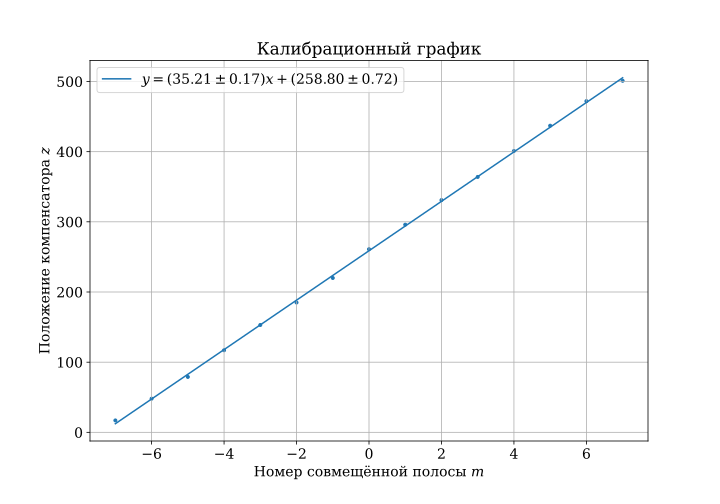
\includegraphics[width=\textwidth]{plot1.png}
\caption{Зависимости амплитуды от частоты и аппроксимация кривых}
\label{graph:1}
\end{center}
\end{figure}

\paragraph{} Полученные значения для добротности $Q_1 = 26.9\pm0.4$ и  $Q_2 = 7.6\pm0.2$.

\subsection{Изучение скорости нарастания и затухания вынужденных колебаний на резонансе}

\paragraph{} Подадим на колебательный контур сигнал в виде цугов. Измерим амплитуды возрастающих и убывающих вынужденных колебаний. Результаты покажем на графике \ref{graph:2}.

\begin{figure} [h]
\begin{center}
\includegraphics[width=\textwidth]{plot2.png}
\caption{Амплитуды нарастающих и затухающих вынужденных колебаний}
\label{graph:2}
\end{center}
\end{figure}

\paragraph{} Найдём логарифмический декремент затухания и нарастания колебаний по формуле:

\[ \Theta = \frac{1}{n} \left( \ln{(U_0 - U_k)} - \ln{(U_0 - U_{k+n})} \right), 
\]

\noindent где $U_0$ -- максимальная амплитуда (в нашем случае $U_0 = 8$), $U_k$ и  $U_{k+n}$ -- амплитуды $k$-го и $k+n$-го колебания. Считая что погрешность $\Delta U_k = \Delta U_{k + n} = \Delta U$, найдём погрешность $\Delta \Theta$:

\[ \Delta \Theta = \frac{\Delta U}{n} \left( \frac{1}{U_0 - U_k} + \frac{1}{U_0 - U_{k+n}} \right).
\]

\noindent Для добротности получаем:

\[ Q = \frac{\pi}{\Theta}, \;\;\; \Delta Q = \frac{\Delta \Theta}{\Theta} Q. 
\]

\paragraph{} Получаем для нарастающих колебаний: $Q_1 = 26.0 \pm 1.4$, $Q_2 = 7.7 \pm 0.7$ ; для убывающих колебаний: $Q_1 = 26.7 \pm 1.3$, $Q_2 = 7.5 \pm 0.7$.

\subsection{Нахождение теоретической добротности}

\paragraph{} Измерим индуктивность, сопротивление и добротность цепи с помощью LCR-7819. При частоте колебаний $\nu = 1.5$ кГц. Получаем $L = 99.63$ мГн, $R = 29.97$ Ом, $Q = 31.33$. Считая, что $C = 0.1$ мкФ, рассчитаем добротность по формуле:

\[ Q = \frac{1}{R} \sqrt{\frac{L}{C}}.
\]

\noindent Взяв $R_1 = 30$ Ом и $R_2 = 130$ Ом, получим: $Q_1 = 33.3$, $Q_2 = 7.7$.


\medskip\hrule\medskip

\section{Выводы}

\paragraph{} Вычисленные несколькими способами добротности:


\begin{center}
\begin{tabular}{|l|l|cccc|}
\hline
\multicolumn{1}{|c|}{\multirow{2}{*}{$R$}} & \multicolumn{1}{c|}{\multirow{2}{*}{$R_\Sigma$}} & \multicolumn{4}{c|}{Q}                                                                                                  \\ \cline{3-6} 
\multicolumn{1}{|c|}{}                     & \multicolumn{1}{c|}{}                            & \multicolumn{1}{c|}{АЧХ} & \multicolumn{1}{c|}{$\Theta \uparrow$} & \multicolumn{1}{c|}{$\Theta \downarrow$} & $f(CRL)$ \\ \hline
0                                          & 30                                               & \multicolumn{1}{l|}{$26.9\pm0.4$}   & \multicolumn{1}{l|}{$26.0 \pm 1.4$}                 & \multicolumn{1}{l|}{$26.7 \pm 1.3$}                   & $33.3 $       \\ \hline
100                                        & 130                                              & \multicolumn{1}{l|}{$7.6\pm0.2$}   & \multicolumn{1}{l|}{$7.7 \pm 0.7$}                 & \multicolumn{1}{l|}{$7.5 \pm 0.7$}                   & $7.7$        \\ \hline
\end{tabular}
\end{center}

Видим, что значения получились похожими, чем показали, что затухание и нарастание, как и АЧХ контура связанны с одной общей добротностью.

\medskip\hrule\medskip

\end{document}
